\documentclass[border=0pt]{standalone}
\usepackage{amsmath,amssymb}
\usepackage{xcolor}
\usepackage{tikz}
\usetikzlibrary{arrows.meta,calc,decorations.pathreplacing,positioning,shapes.geometric,backgrounds}
\definecolor{c1}{RGB}{0,114,178}
\definecolor{c2}{RGB}{230,159,0}
\definecolor{c3}{RGB}{0,158,115}
\definecolor{cr}{RGB}{213,94,0}
\tikzset{every picture/.append style={show background rectangle,
    background rectangle/.style={fill=white}, inner frame sep=8pt}}
\newcommand{\roll}{\mathcal{R}}
\begin{document}
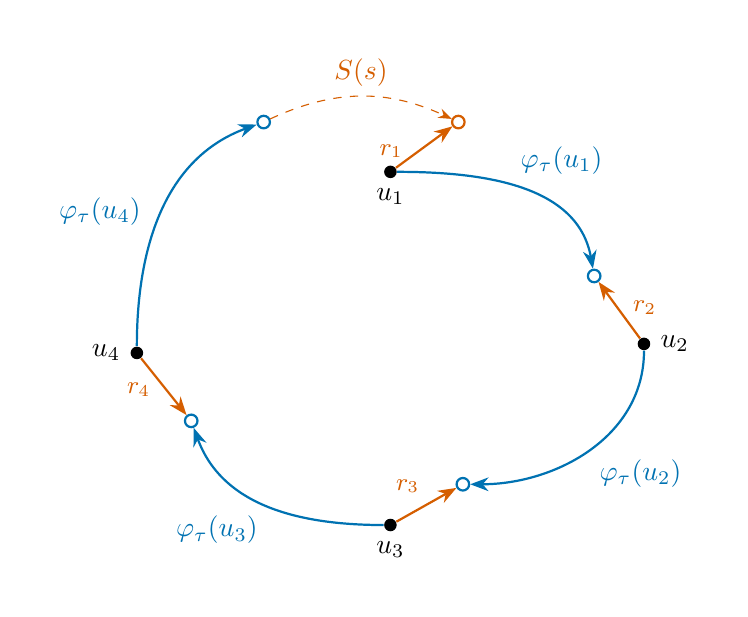
\begin{tikzpicture}[>=Stealth, scale=1.15,
      seed/.style={circle, fill=black, inner sep=1.6pt},
      end/.style={circle, draw=c1, fill=white, inner sep=1.6pt, thick}]
    % seeds
    \node[seed, label=below:{$u_1$}]      (u1) at (0, 2.0) {};
    \node[seed, label=right:{$u_2$}]      (u2) at (2.8, 0.1) {};
    \node[seed, label=below:{$u_3$}]      (u3) at (0, -1.9) {};
    \node[seed, label=left:{$u_4$}]       (u4) at (-2.8, 0.0) {};
    % ends of the segments
    \node[end] (e1) at (2.25, 0.85) {};
    \node[end] (e2) at (0.8, -1.45) {};
    \node[end] (e3) at (-2.2, -0.75) {};
    \node[end] (e4) at (-1.4, 2.55) {};
    \node[end, draw=cr] (w) at (0.75, 2.55) {};
    % segments
    \draw[->, c1, thick] (u1) to[out=0, in=100] node[pos=0.45, above right] {$\varphi_\tau(u_1)$} (e1);
    \draw[->, c1, thick] (u2) to[out=-90, in=0] node[pos=0.5, below right] {$\varphi_\tau(u_2)$} (e2);
    \draw[->, c1, thick] (u3) to[out=180, in=-70] node[pos=0.5, below left] {$\varphi_\tau(u_3)$} (e3);
    \draw[->, c1, thick] (u4) to[out=90, in=200] node[pos=0.5, left=4pt] {$\varphi_\tau(u_4)$} (e4);
    % shift of the last end
    \draw[->, cr, dashed] (e4) to[out=25, in=155] node[above] {$S(s)$} (w);
    % residuals
    \draw[->, cr, thick] (u2) -- (e1) node[pos=0.55, right=2pt] {\small $r_2$};
    \draw[->, cr, thick] (u3) -- (e2) node[pos=0.55, above left=0pt] {\small $r_3$};
    \draw[->, cr, thick] (u4) -- (e3) node[pos=0.55, left=2pt] {\small $r_4$};
    \draw[->, cr, thick] (u1) -- (w)  node[pos=0.4, left=2pt] {\small $r_1$};
  \end{tikzpicture}
\end{document}
